% agent-rewind: project report, Option 5.
% Format: 10pt on 12pt leading, two columns, Times-like, 7 x 9 in text block, numbered pages.
% Build: `tectonic main.tex` (or `latexmk -pdf main.tex`) from this folder.
\documentclass[10pt,twocolumn,letterpaper]{article}

\usepackage[T1]{fontenc}
\usepackage{newtxtext,newtxmath}
\usepackage[textwidth=7in,textheight=9in,columnsep=0.33in,centering]{geometry}
\usepackage{graphicx}
\usepackage{booktabs}
\usepackage{tabularx}
\usepackage{multirow}
\usepackage{xcolor}
\usepackage{tikz}
\usetikzlibrary{arrows.meta,positioning,fit,backgrounds,calc}
\usepackage[font=small,labelfont=bf,skip=4pt]{caption}
\usepackage{enumitem}
\usepackage{microtype}
\usepackage[hidelinks]{hyperref}

\setlist{nosep,leftmargin=*}
\setlength{\textfloatsep}{8pt plus 2pt minus 2pt}
\setlength{\dbltextfloatsep}{8pt plus 2pt minus 2pt}
\pagestyle{plain}
\raggedbottom

\newcommand{\sys}{\textsc{Agent-Rewind}}
\newcommand{\pmsd}[2]{#1\,{\scriptsize$\pm$\,#2}}
\newcommand{\verdict}[1]{\textit{#1}}
\definecolor{accent}{HTML}{0072B2}
\definecolor{warn}{HTML}{D55E00}
\definecolor{soft}{HTML}{E8F1F8}

\title{\Large\bfseries Provenance All the Way Down: Selective Recovery\\for Multi-Agent LLM Workflows}
\author{Yitang Gao \quad Qinlin Chen \quad Xueru Song \quad Kai Zhang\\ \normalsize University of California, San Diego}
\date{}

\begin{document}
\maketitle

\begin{abstract}
When an agent in a multi-agent workflow produces a wrong fact, a stale lookup or
an injected instruction, every later step that read it is suspect, and some of
those steps have already acted on the world. We ask whether tracking the exact
dependencies between agent results makes recovery both cheap and safe. \sys{}
records, for every step, the ordered \emph{(path, Merkle hash)} pairs it read
from one hierarchical namespace of messages, shared state, files and tool
results. Recovery re-executes the workflow and reuses every step whose recorded
reads still verify; early cutoff, precision tiers and dynamic branching follow
from that single rule. The same provenance then decides which \emph{tokens} a
rerun must re-decode (speculative replay against the step's old output) and
which \emph{audits} must be redone. On four workloads with a local 7B model
(2{,}215 measured cells), selective recovery reruns 5.0 of 24 steps where
restart reruns 22.5, halves W1 recovery time (16.1\,s vs 32.4\,s), and an
intent-diff effect layer cuts re-sent irreversible calls from 3.0 to 0.33 per
recovery. Replay decodes 9--65\% of the tokens of a plain rerun with identical
output on short prompts, but does not reliably save wall time. Scoped audits do
\emph{not} match always-verify detection; their cached verdicts do cut
post-recovery audit tokens by 69\%. We report each claim with the verdict the
data supports, including the negative ones.
\end{abstract}

% ---------------------------------------------------------------------------
\section{Introduction}

Multi-agent LLM systems split a task across roles: a \emph{researcher} gathers
facts, a \emph{planner} decides, an \emph{executor} calls tools. Failures in such
systems rarely stay local~\cite{cemri2025why,huang2025resilience}: a hallucinated
room capacity becomes a booking, a booking becomes an e-mail. Once a faulty
result is identified, the operator faces three questions:
(1)~\emph{propagation}: which later results and effects did it influence?
(2)~\emph{recovery}: what is the least work that restores a correct state?
(3)~\emph{safety}: which effects can be undone, and which must never be repeated?

The default answers are coarse. Restart redoes everything and repeats every
side effect. Checkpoint rollback~\cite{li2025agentgit} redoes the whole
time-order suffix after the fault, including work that never read the faulty
value. Always-verify pays a model call on every output in every run. Systems
research has better answers for other domains: build systems rerun a target
only when an input hash changed~\cite{mokhov2018build,mitchell2012shake},
intrusion-recovery systems re-execute only actions that depend on an
attack~\cite{kim2010retro}, and sagas compensate effects that cannot be rolled
back~\cite{garcia1987sagas}. This project asks whether those ideas carry over to
LLM agents, whose steps are expensive, non-idempotent and act on the world.

\paragraph{Contributions.}
\begin{itemize}
\item \textbf{Verifying traces over a Merkle namespace} (\S\ref{sec:design}). One
  engine runs clean, faulty and recovery executions. A step is reused iff every
  recorded read hash still matches. Precision versus bookkeeping becomes a
  single depth knob (agent $\to$ step $\to$ artifact $\to$ field).
\item \textbf{An intent-diff effect layer} with idempotency keys, compensation
  and an outbox, so recovery re-sends only effects whose intent changed.
\item \textbf{Provenance inside a step}: speculative replay (M1) uses the faulty
  run's own output as a draft; atom-structured reasoning (M2) makes reruns
  local; scoped, cached audits (M3) and cone-cost audit placement (M4) treat
  verification as graph nodes.
\item \textbf{An honest evaluation} (\S\ref{sec:eval}) on four workloads, including
  two scenarios ported from TAMAS~\cite{kavathekar2025tamas}, with a local
  7B model on one laptop. Each claim gets a verdict: supported, partly
  supported, inconclusive, or not supported.
\end{itemize}

% ---------------------------------------------------------------------------
\section{Problem Setting and Fault Model}
\label{sec:problem}

A \emph{workflow} is a set of steps run by agents. Steps read and write state and
call tools. A run is \emph{correct} when its final outcome and every final
artifact equal those of the clean run. We inject one fault per run at a chosen
step and stage:
\emph{wrong} (a plausible but false value), \emph{stale} (an outdated value),
\emph{timeout} (missing value), and \emph{malicious} (an injected instruction,
or a Byzantine agent). Accidental and adversarial faults are reported apart.

We \textbf{separate detection from recovery}: every
recovery method is told the identity of the faulty result, so recovery is judged
on its own. Automated detection (audits) is scored separately as a detector,
with false positives and misses. A fault that is read but changes nothing is
flagged as non-propagating rather than counted as robustness.

Tool effects carry MCP-style classes~\cite{mcp}: \texttt{read},
\texttt{idempotent}, \texttt{compensable} (a booking can be cancelled), and
\texttt{irreversible} (a sent e-mail stays sent; it is reported as
\emph{leaked}, never counted as recovered).

% ---------------------------------------------------------------------------
\section{Design}
\label{sec:design}

\begin{figure*}[t]
\centering
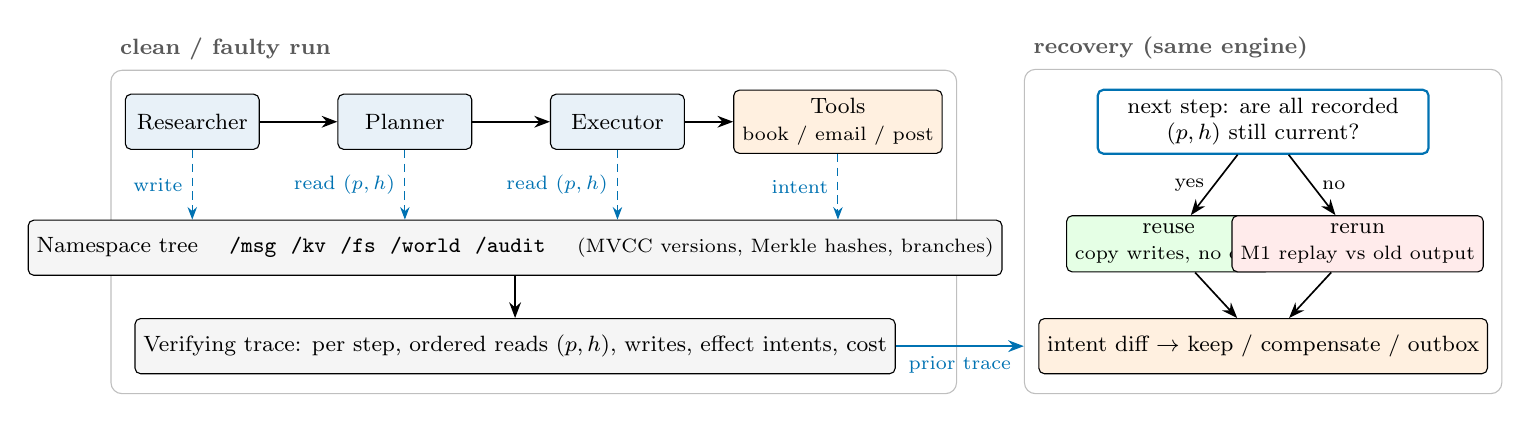
\begin{tikzpicture}[
  font=\footnotesize,
  box/.style={draw, rounded corners=2pt, align=center, minimum height=7mm, inner sep=3pt},
  agent/.style={box, fill=soft, minimum width=17mm},
  store/.style={box, fill=gray!8},
  arr/.style={-{Stealth[length=2mm]}, semithick},
  dep/.style={-{Stealth[length=1.6mm]}, densely dashed, accent},
  panel/.style={draw=gray!50, rounded corners=4pt, inner sep=5pt},
  ttl/.style={font=\footnotesize\bfseries, text=gray!70!black, anchor=south west},
]
% ---- left panel: normal execution ----
\node[agent] (res) at (0,0) {Researcher};
\node[agent] (plan) at (2.7,0) {Planner};
\node[agent] (exe) at (5.4,0) {Executor};
\node[box, fill=orange!12] (tools) at (8.2,0) {Tools\\{\scriptsize book / email / post}};
\draw[arr] (res) -- (plan);
\draw[arr] (plan) -- (exe);
\draw[arr] (exe) -- (tools);
\node[store, minimum width=88mm] (ns) at (4.1,-1.6)
  {Namespace tree \quad \texttt{/msg}\; \texttt{/kv}\; \texttt{/fs}\; \texttt{/world}\; \texttt{/audit}
   \quad{\scriptsize(MVCC versions, Merkle hashes, branches)}};
\draw[dep] (res) -- node[left]{\scriptsize write} (res |- ns.north);
\draw[dep] (plan) -- node[left]{\scriptsize read $(p,h)$} (plan |- ns.north);
\draw[dep] (exe) -- node[left]{\scriptsize read $(p,h)$} (exe |- ns.north);
\draw[dep] (tools) -- node[left]{\scriptsize intent} (tools |- ns.north);
\node[store, minimum width=88mm] (trace) at (4.1,-2.85)
  {Verifying trace: per step, ordered reads $(p,h)$, writes, effect intents, cost};
\draw[arr] (ns) -- (trace);
\begin{scope}[on background layer]
\node[panel, fit=(res)(tools)(trace), inner ysep=7pt] (L) {};
\end{scope}
\node[ttl] at (L.north west) {clean / faulty run};
% ---- right panel: recovery ----
\node[box, draw=accent, thick, minimum width=42mm] (q) at (13.6,0)
  {next step: are all recorded\\ $(p,h)$ still current?};
\node[box, fill=green!10, minimum width=19mm] (reuse) at (12.4,-1.55) {reuse\\{\scriptsize copy writes, no call}};
\node[box, fill=red!8, minimum width=19mm] (rerun) at (14.8,-1.55) {rerun\\{\scriptsize M1 replay vs old output}};
\draw[arr] (q) -- node[left]{\scriptsize yes} (reuse);
\draw[arr] (q) -- node[right]{\scriptsize no} (rerun);
\node[box, fill=orange!12, minimum width=42mm] (eff) at (13.6,-2.85)
  {intent diff $\to$ keep / compensate / outbox};
\draw[arr] (reuse) -- (eff);
\draw[arr] (rerun) -- (eff);
\begin{scope}[on background layer]
\node[panel, fit=(q)(reuse)(rerun)(eff), inner ysep=7pt] (R) {};
\end{scope}
\node[ttl] at (R.north west) {recovery (same engine)};
\draw[arr, accent, thick] (trace.east) -- node[below, font=\scriptsize]{prior trace} (eff.west -| R.west);
\end{tikzpicture}
\caption{\sys{} at a glance. Agents read and write one versioned namespace; each
step's ordered read hashes form a verifying trace. On recovery a step is reused
iff its reads still verify; otherwise it reruns, decoding against its old output
(M1). Effects are reconciled by intent, not undone and redone.}
\label{fig:arch}
\end{figure*}

\subsection{One namespace, Merkle hashes}
All state a step can touch is a node in one tree: messages
(\texttt{/msg/<step>/...}), shared state (\texttt{/kv}), files (\texttt{/fs},
backed by a git workspace whose tree objects are already Merkle trees), tool
results keyed by intent (\texttt{/world}) and audit verdicts (\texttt{/audit}).
JSON values are subtrees, so \texttt{/msg/planner/plan/agenda/items/2} is a valid
path. Writes append MVCC versions; a recovery run continues on a new branch, so
the faulty and recovered runs share every version they agree on.

A read is recorded as $(\mathrm{cut}(p,d), \mathrm{hash}(\mathrm{cut}(p,d)))$.
Because an ancestor's hash changes whenever anything below it changes, a coarser
cut can only over-invalidate, never miss a change. The four precision tiers the
brief asks about are depth cuts $d$ of the same tree (agent $d{=}2$, step $3$,
artifact $4$, field $=$ full path).

\subsection{Recovery as re-execution against a trace}
Every method runs the same loop (Fig.~\ref{fig:arch}). For each step in
(dynamic) workflow order, if the step is not marked dirty and all its recorded
read hashes match the current store, its writes are copied forward and its
intents kept, with no model call. Otherwise it reruns. Methods differ only in
what they mark dirty: \emph{restart} marks everything, \emph{rollback} marks
the time-order suffix from the fault, \emph{selective} marks only the faulty
producer. Several properties then come for free:
\begin{itemize}
\item \textbf{Early cutoff.} If a rerun reproduces the same value, downstream
  hashes match and propagation stops, as in Shake~\cite{mitchell2012shake}.
  An \emph{exact} or \emph{canonical} (normalised JSON) hash sets the cutoff tier.
\item \textbf{Write-set changes.} If a rerun no longer writes a key a later step
  read, that key now hashes to $\bot$ and the reader reruns. A static
  ``changed-set'' DAG would miss this.
\item \textbf{Branch flips.} Steps that no longer run become \emph{orphans}; their
  effects are reconciled against an empty intent list.
\end{itemize}

\subsection{Effects: intents, not undo-redo}
Each tool call becomes an intent keyed by $h(\text{step},\text{tool},\text{args})$.
After a rerun, the old and new intent lists are diffed: identical intents are
kept, removed compensable ones are compensated, and irreversible ones are held
in an \emph{outbox} until the run commits. Policies \texttt{naive} (undo
everything, redo everything), \texttt{diff} and \texttt{diff+outbox} are
compared in \S\ref{sec:effects}.

\subsection{Provenance inside a step and for audits}
\textbf{M1 speculative replay.} A rerun step prefills its new prompt and feeds its
old output as a draft; tokens are accepted while the greedy argmax agrees, with
n-gram resynchronisation after a divergence (the LLMA idea~\cite{yang2023llma}
applied to the step's own output). Under greedy decoding the result equals a
plain decode~\cite{leviathan2023fast}, up to floating-point ties, which we
re-verify within a margin.
\textbf{M2 atoms.} Outputs are a canonical list of \emph{atoms} (one per input
group, each citing the paths it uses) plus an answer, so a changed input
perturbs mainly its own atom.
\textbf{M3 scoped, cached audits.} An audit checks one atom against only the
values it read, and its verdict is stored at \texttt{/audit/...} keyed by the
atom and source hashes, so the step engine re-audits only what changed.
\textbf{M4 placement.} Audit an atom when
$\mathit{risk}\times\mathit{cost}(\mathit{cone})+w\cdot[\text{reaches irreversible}]$
exceeds the audit cost, with risk from token confidence~\cite{fu2025deepconf}.

% ---------------------------------------------------------------------------
\section{Implementation}
\label{sec:impl}

\sys{} is about 5{,}600 lines of Python (including tests). The core
(\texttt{store}, \texttt{engine}, \texttt{deps}, \texttt{cutoff},
\texttt{effects}) uses only the standard library, with a SQLite journal. Real
models run in-process through \texttt{llama-cpp-python} 0.3.36 on Metal, because
M1 needs per-position logits and KV-cache cropping that an HTTP server does not
expose. Model output is grammar-constrained JSON at temperature~0.
A scripted model drives the large sweeps and the property tests.

\paragraph{Workloads.}
\textbf{W1} booking: researcher $\to$ planner $\to$ executor scheduling $k$
meetings over shared team facts (14 steps, 6 LLM calls; \texttt{calendar.book}
is compensable, \texttt{email.send} irreversible).
\textbf{W2} synthetic DAGs (24 steps) varying layers, fan-in, shared keys and
effect mix, scripted.
\textbf{W3} a code fix in a git workspace, checked by unit tests (non-LLM file
state). \textbf{W4} two TAMAS~\cite{kavathekar2025tamas} scenarios ported as
native workflows: Byzantine agents (\texttt{w4.byz}) and indirect prompt
injection (\texttt{w4.ipi}), whose effects are social-media posts.

\paragraph{Platform.} One Apple M5 Pro laptop (24\,GB), Qwen2.5-7B-Instruct
Q4\_K\_M, greedy decoding. The full grid (540 cells) ran in 2.8\,h with a peak
RSS of 6.3\,GB and zero errors; Phase~1 added 1{,}675 cells.

% ---------------------------------------------------------------------------
\section{Evaluation}
\label{sec:eval}

We report mean\,$\pm$\,sd. Repeats are scenario variants (greedy decoding is
deterministic), so the noise floor is the clean-vs-clean spread: all four
workloads succeed 3/3 clean, and a difference of one cell in ten (0.1) is inside
that floor. Correctness uses \texttt{ok\_recovered}, since W1's irreversible
e-mails make its final state unrecoverable by design.

\subsection{Propagation (Phase 1)}
Every injected fault is read downstream (rate 1.0 for all 24 fault$\times$workload
pairs). Table~\ref{tab:prop} shows that reach varies widely: a wrong W1 capacity
taints 9 of 14 steps and reaches both the booking and the irreversible e-mail;
an injected agenda taints only 3 but sends an unauthorised e-mail. Three 7B
faults are read yet \emph{do not} change the outcome (W3 \texttt{inject\_issue},
W4 \texttt{byz\_factcheck} on both scenarios); the scripted model propagates
them all, so non-propagation is a property of the model, and we flag rather
than count it.

\begin{table}[t]
\centering\small
\caption{Fault propagation with the 7B model (E1, $n{=}3$ each).}
\label{tab:prop}
\setlength{\tabcolsep}{3.5pt}
\begin{tabular}{@{}llccc@{}}
\toprule
WL & fault (class) & outcome chg. & steps hit & irrev. \\
\midrule
W1 & wrong\_capacity (acc.) & 1.00 & 9/14 & 3 \\
W1 & stale\_capacity (acc.) & 0.67 & 9/14 & 3 \\
W1 & inject\_agenda (adv.) & 1.00 & 3/14 & 3 \\
W3 & wrong\_issue (acc.) & 1.00 & 3/5 & 0 \\
W3 & inject\_issue (adv.) & \textcolor{warn}{0.00} & 3/5 & 0 \\
W4.byz & byz\_distribute (adv.) & 1.00 & 1/6 & 1 \\
W4.byz & byz\_factcheck (adv.) & \textcolor{warn}{0.00} & 3/6 & 2 \\
W4.ipi & inject\_item (adv.) & 0.33 & 4/6 & 1.3 \\
\bottomrule
\end{tabular}
\end{table}


\subsection{P1: reruns follow the cone, not the suffix}
\label{sec:p1}
On W2 (225 cells per method) restart reruns \pmsd{22.5}{1.2} of 24 steps,
rollback \pmsd{13.3}{5.9}, and selective \pmsd{5.0}{4.5}, which is
\pmsd{1.01}{0.68}$\times$ the size of $\mathrm{cone}(f)\cup\{f\}$
(Fig.~\ref{fig:cone}). Selective tracks the cone at every fault position;
rollback tracks the suffix, so its advantage over restart vanishes for early
faults. The subset property holds in 203/225 cells. Of the 22 exceptions, 14
only add steps that never ran in the faulty run (the fault changed control flow),
and 13 rerun a step outside the cone, concentrated at shared-key faults.
\verdict{Verdict: supported as an aggregate, not as an exact subset property.}

\begin{figure*}[t]
\centering
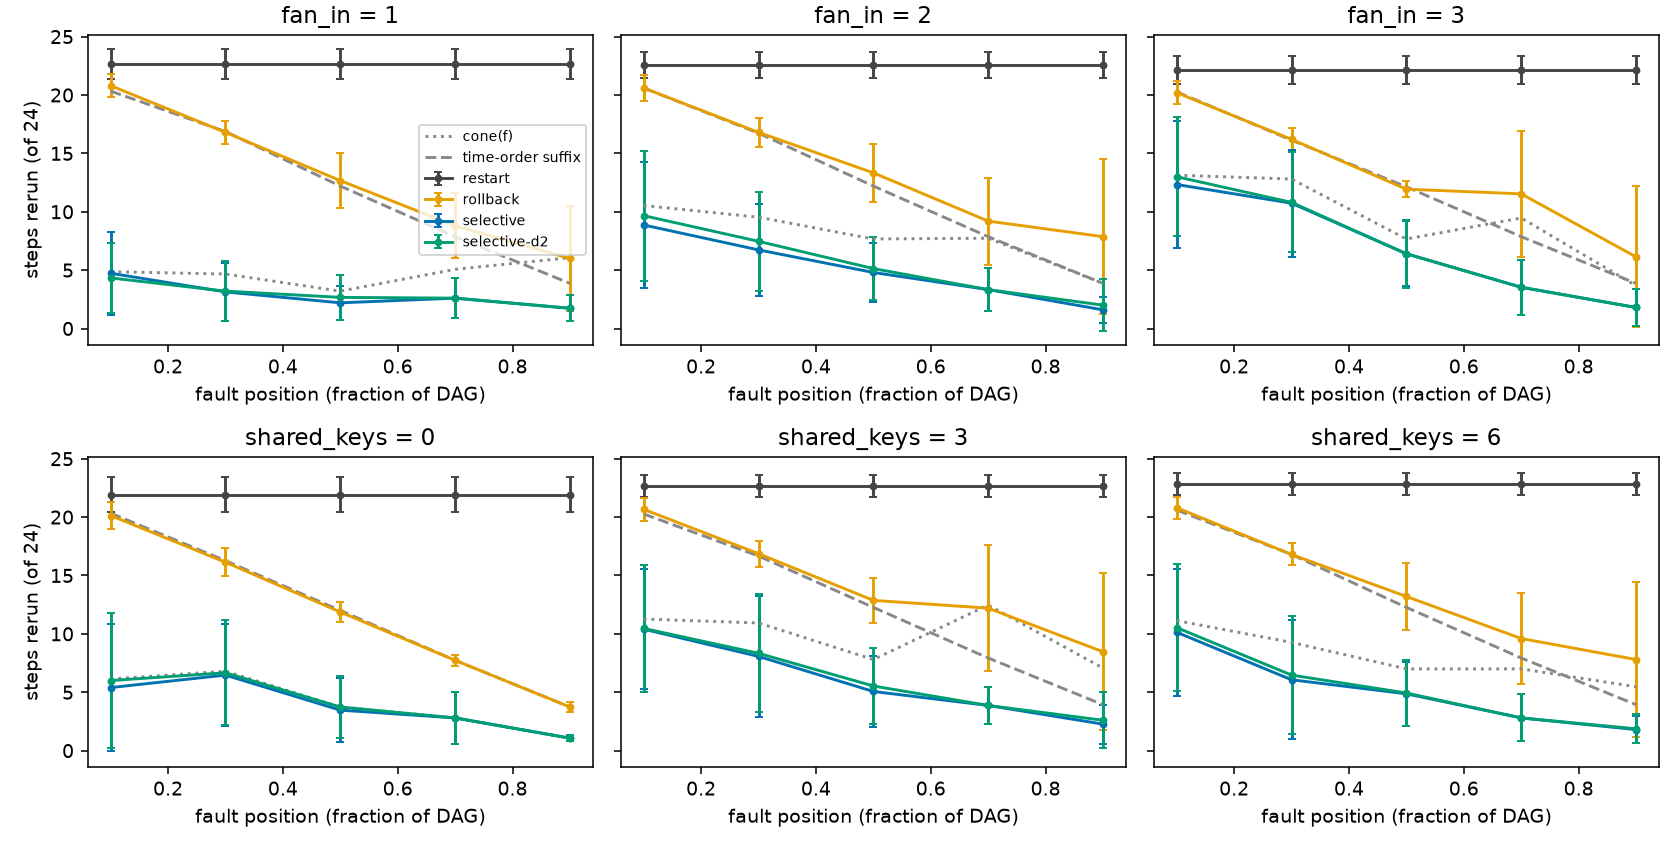
\includegraphics[width=\textwidth]{figures/fig1_cone_vs_suffix.png}
\caption{P1 (E2, W2 scripted). Steps rerun against fault position. Selective
recovery (blue/green) follows the dependency cone (dotted); rollback (orange)
follows the time-order suffix (dashed); restart is flat near 22.5.}
\label{fig:cone}
\end{figure*}

\begin{figure*}[t]
\centering
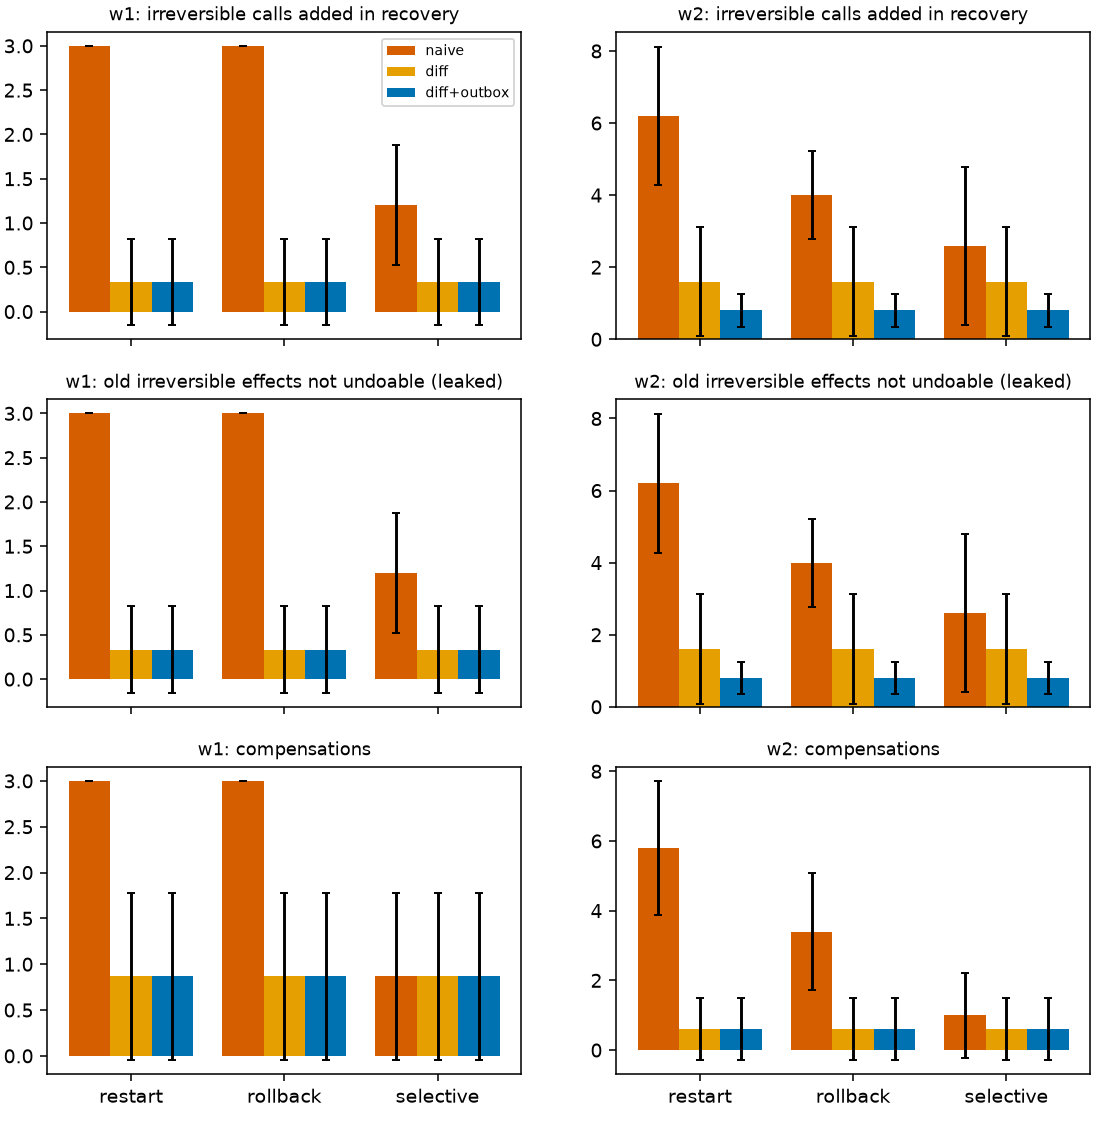
\includegraphics[width=0.62\textwidth]{figures/fig3_effects.png}
\caption{P3 (E4). Compensations and irreversible calls added during recovery by
effect policy, for W1 (left) and W2 (right). Rows: irreversible calls added,
old irreversible effects that cannot be undone (leaked), compensations. Intent
diff removes most undo-redo churn.}
\label{fig:effects}
\end{figure*}

\subsection{P2: precision versus bookkeeping}
Finer cuts rerun fewer steps on W2: agent \pmsd{8.87}{4.56}, step
\pmsd{6.67}{4.70}, artifact \pmsd{6.67}{4.70}, field \pmsd{6.27}{4.35}. Paired
agent-minus-field savings are 2.6 (W2) and 3.4 (W1) steps, and no cell is
worse. The \emph{canonical} cutoff never helps (807 vs 807 total reruns).
Bookkeeping cost, however, did not rise measurably with depth in the scripted
proxy (tracked run 1.34\,ms agent vs 1.22\,ms field), and was not measured on
real runs. \verdict{Verdict: precision half supported; the trade-off is
inconclusive.}

\subsection{P3: effect safety}
\label{sec:effects}
On W1 (Fig.~\ref{fig:effects}), naive restart compensates 3.0 bookings and re-sends
3.0 irreversible calls per recovery. With intent diff, compensations drop to
\pmsd{0.87}{0.92} and re-sent irreversible calls to \pmsd{0.33}{0.49}, the same
for all three methods (effects are retained by intent key). On W2 the outbox
matters: re-sent irreversible calls fall $6.2\to1.6\to0.8$ (naive, diff,
diff+outbox). Effects that had already left the system before the fault was
known remain \emph{leaked} (0.33 on W1). \verdict{Verdict: supported for
compensations and re-sent calls; ``zero duplicates'' was not directly counted.}

\subsection{C-A, C-B: replay and structure}
\begin{figure*}[t]
\centering
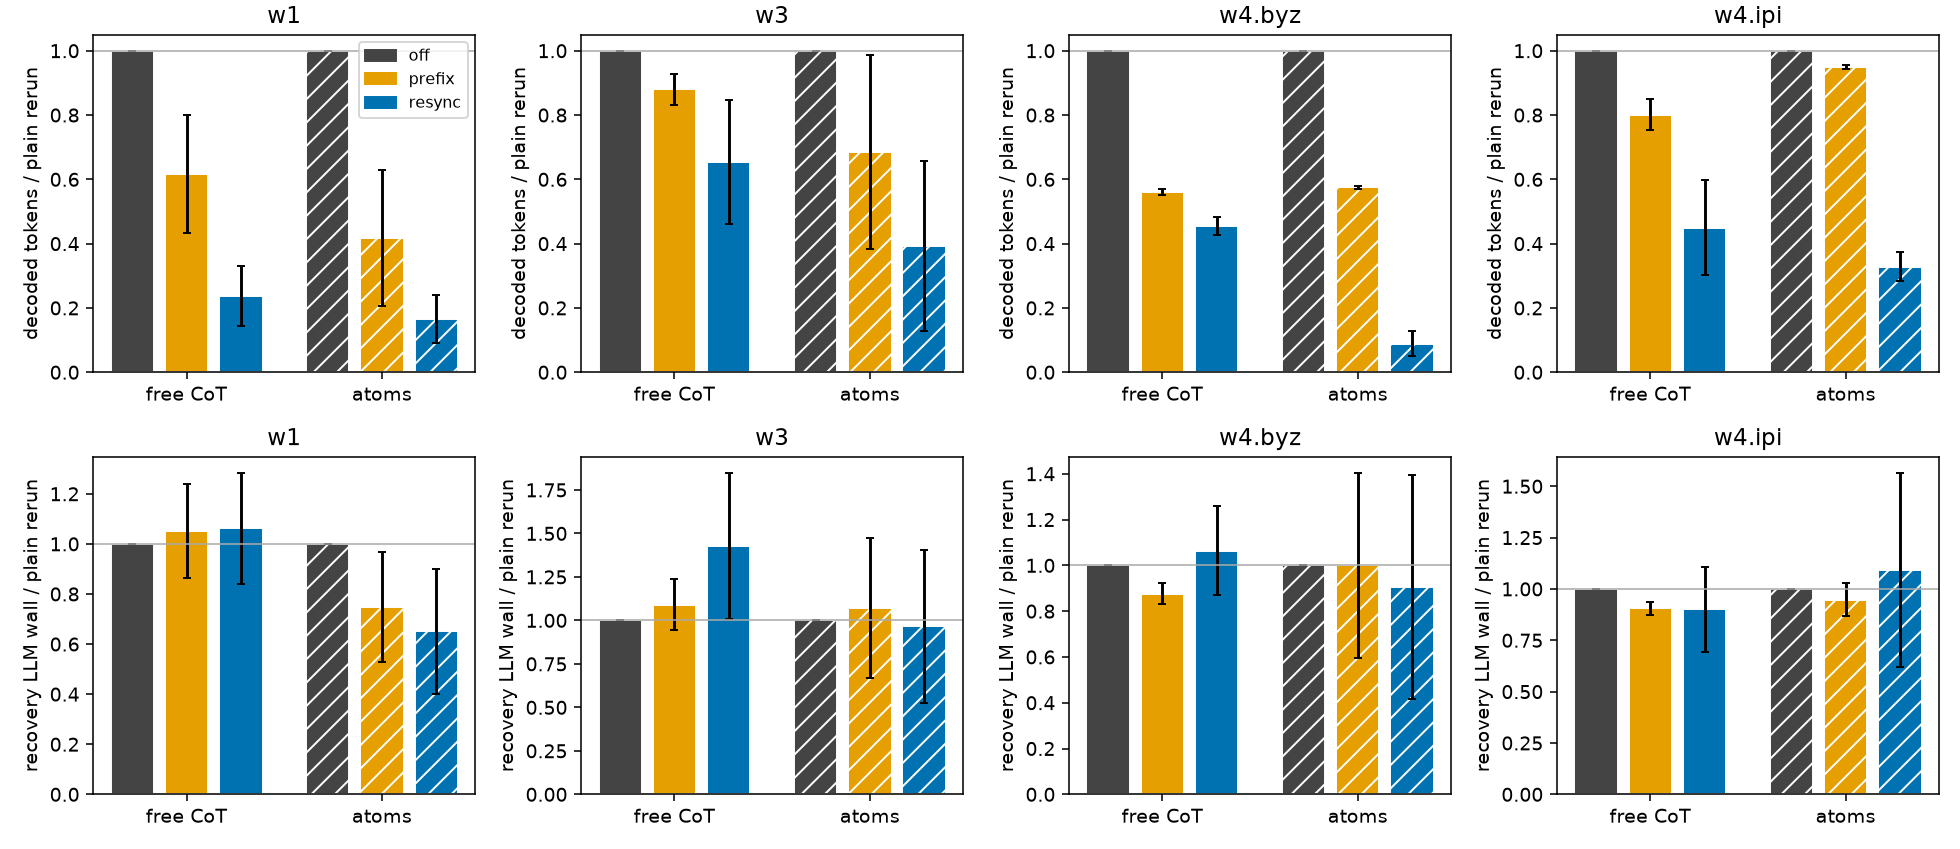
\includegraphics[width=\textwidth]{figures/fig4_replay.png}
\caption{C-A (E5, 7B). Top: decoded tokens of a replayed rerun relative to a
plain rerun. Bottom: recovery LLM wall time relative to a plain rerun. Hatched
bars use atom-structured output (M2).}
\label{fig:replay}
\end{figure*}
Replay with resynchronisation decodes 0.24 (W1), 0.65 (W3), 0.46 (W4.byz) and
0.45 (W4.ipi) of a plain rerun's tokens with free chain-of-thought, and 0.17,
0.39, 0.09 and 0.33 with atoms (Fig.~\ref{fig:replay}). In a separate check,
74/74 replays were token-identical to plain greedy decoding on prompts of at
most 512 tokens; longer prompts (W3, about 650 tokens) only showed equal output
lengths and outcomes. Wall time is another story: ratios are 1.06 (W1 CoT),
1.43 (W3 CoT), 0.65 (W1 atoms) and 0.97 (W3 atoms), because re-verifying
near-ties on a 7B model costs about as much as it saves. Atoms raise replay
acceptance on all four workloads (e.g., W4.byz 0.91 vs 0.55), but cost more
tokens per live call, and the break-even fault rate $p^*$ is bounded only for
W4.byz (0.15, 95\% CI 0.09--0.22, $n{=}3$).
\verdict{Verdicts: C-A token saving and equality (short prompts) supported, wall
time not; C-B acceptance supported, break-even inconclusive.}

\subsection{C-C, C-D: audits}
\begin{table}[t]
\centering\small
\caption{Audits as detectors (E7, 7B). Detection with Wilson 95\% CI; tokens
per faulty run; audit tokens spent re-checking after recovery.}
\label{tab:audit}
\setlength{\tabcolsep}{3pt}
\begin{tabular}{@{}llccc@{}}
\toprule
WL & policy & detected & tok/run & re-audit tok \\
\midrule
\multirow{4}{*}{W1} & always   & 1.00 [.72,1] & 1239 & 1224 \\
                    & M3       & 0.40 [.17,.69] & 1211 & 1206 \\
                    & M3+cache & 0.40 [.17,.69] & 1211 & \textbf{379} \\
                    & M3+M4    & 0.30 [.11,.60] & \textbf{273} & 147 \\
\midrule
\multirow{2}{*}{W3} & always   & 1.00 [.57,1] & 589 & 586 \\
                    & M3+M4    & 0.00 [0,.43] & 0 & 0 \\
\midrule
\multirow{2}{*}{W4.byz} & always & 1.00 [.44,1] & 656 & 658 \\
                        & M3+cache & 1.00 [.44,1] & 524 & 171 \\
\bottomrule
\end{tabular}
\end{table}
Scoping alone does not deliver the claimed saving (Table~\ref{tab:audit}): M3
spends almost as many tokens as always-verify on W1 ($-2\%$) and detects far
less (0.40 vs 1.00; it misses the injected agenda 0/5). What \emph{does} work is
treating verdicts as cached graph nodes: after recovery, W1 re-audits drop from
15.0 to \pmsd{4.7}{3.8} and their tokens by 69\%. Cone-cost placement (M4) cuts
tokens by 77\% but misses more faults on three of four workloads.
\verdict{Verdicts: C-C detection not supported, cache reuse supported; C-D
inconclusive.}

\subsection{End-to-end (E8)}
\begin{table}[t]
\centering\small
\caption{End-to-end recovery (E8, 7B). Steps rerun, recovery LLM wall time,
decoded tokens and correctness. $^\dagger$W1 free-CoT rows fail even when clean
(0/5), so W1 correctness compares styles, not methods.}
\label{tab:e2e}
\setlength{\tabcolsep}{2.6pt}
\begin{tabular}{@{}llcccc@{}}
\toprule
WL & method & rerun & wall s & dec. tok & ok \\
\midrule
\multirow{4}{*}{W1} & restart   & 14.0 & 32.4 & 621 & 0.00$^\dagger$ \\
                    & rollback  & 12.5 & 32.4 & 621 & 0.00$^\dagger$ \\
                    & selective & 4.3 & 16.1 & 316 & 0.00$^\dagger$ \\
                    & sel.+M1+M2 & 6.3 & \textbf{13.8} & \textbf{85} & 0.80 \\
\midrule
\multirow{3}{*}{W3} & restart   & 5.0 & 6.2 & 121 & 0.80 \\
                    & selective & 4.0 & 6.3 & 123 & 0.70 \\
                    & sel.+M1+M2 & 4.0 & 7.8 & 66 & 0.90 \\
\midrule
\multirow{3}{*}{W4.byz} & restart & 6.0 & 13.1 & 261 & 1.00 \\
                        & selective & 4.0 & 13.1 & 261 & 1.00 \\
                        & sel.+M1+M2 & 2.0 & \textbf{7.3} & \textbf{16} & 1.00 \\
\bottomrule
\end{tabular}
\end{table}
Table~\ref{tab:e2e} combines the pieces. On W1, selective recovery reruns 4.3
of 14 steps and halves recovery time against restart; adding replay and atoms
cuts decoded tokens from 316 to 85. On W4.byz the full stack reruns 2 of 6 steps
and decodes 16 tokens instead of 261. W3 is small (5 steps, one LLM call), so
there is little to save, and correctness differences there are inside the
one-cell noise floor. Unauthorised actions (W1 \texttt{inject\_agenda}) occur
once per faulty run under every method: recovery cannot recall an e-mail that
left before the fault was known, which argues for gating irreversible effects
on audits \emph{before} release.

% ---------------------------------------------------------------------------
\section{Related Work}
\label{sec:related}

\textbf{Failures in multi-agent systems.} MAST~\cite{cemri2025why} catalogues
failure modes; failure attribution~\cite{zhang2025which} and resilience
studies~\cite{huang2025resilience} show detection is hard, which motivates
scoring detection apart. TAMAS~\cite{kavathekar2025tamas} and
A2ASecBench~\cite{li2026a2asecbench} supply adversarial scenarios; we port two
TAMAS scenarios.
\textbf{Rollback for agents.} AgentGit~\cite{li2025agentgit} brings git-style
commits and branching to agent state, recovering in time order; we recover by
dependency and add effect classes. Sherlock~\cite{ro2025sherlock} places
verifiers and speculates ahead of them; SagaLLM~\cite{chang2025sagallm} adds
saga-style compensation to planning; dependency-guided rollback
repair~\cite{wang2026rollback} targets memory-augmented agents.
\textbf{Systems foundations.} Retro~\cite{kim2010retro} pioneered selective
re-execution for intrusion recovery; build systems contribute verifying traces
and early cutoff~\cite{mokhov2018build,mitchell2012shake}; lineage-based
recovery dates to RDDs~\cite{zaharia2012rdd}; sagas~\cite{garcia1987sagas}
compensate long transactions.
\textbf{Decoding reuse.} Speculative decoding~\cite{leviathan2023fast} and
reference-copying~\cite{yang2023llma} accelerate generation with drafts; we use
the faulty run's own output as the draft. MiniCheck~\cite{tang2024minicheck} and
DeepConf~\cite{fu2025deepconf} inform the audit checker and risk score.

% ---------------------------------------------------------------------------
\section{Experience, Limitations and Dead Ends}
\label{sec:experience}

\begin{itemize}
\item \textbf{Free-form CoT is not a clean baseline.} W1 with free
  chain-of-thought fails 0/5 even without faults, while atoms succeed 4/5. This
  confounds W1's method comparison with output style; the fix is to rerun
  restart/rollback/selective with atoms.
\item \textbf{Floating-point ties break ``lossless'' replay.} Batched and
  sequential evaluation disagree on near-ties; the first replay attempt matched
  plain decoding only 87.8\% of the time. Re-verifying tokens within a 0.3
  logit margin restored 74/74 identity, at a wall-time cost that cancels most
  of M1's savings on a 7B model.
\item \textbf{Canonical cutoff never fired} beyond exact hashes, because
  constrained JSON output is already canonical.
\item \textbf{Budget cuts.} The 1.5B model was unusable on W1 (2/5 clean), so
  the full grid is 7B only; W4 has 3 repeats; the split-atoms arm and the
  MiniCheck ablation were not run. Injected atom faults keep their original
  confidence, so M4's risk score cannot see them.
\item \textbf{Not yet measured:} tracking overhead on real runs and reuse
  validity by sampled scratch reruns; both are Phase~2 work.
\end{itemize}

% ---------------------------------------------------------------------------
\section{Conclusion}
Recording what each agent step actually read, as hashes in one namespace, turns
recovery into re-execution against a verifying trace. On a laptop-scale study
this reruns the dependency cone instead of the suffix, halves recovery time on
the booking workflow and removes most duplicated side effects. Pushing the same
provenance inside a step saves decoded tokens but not reliably wall time, and
scoping audits to provenance saves re-audits after recovery but does not replace
always-verify as a detector. The clearest lesson is about irreversible effects:
no recovery method can recall them, so verification belongs on the backward
cone of an effect, before it leaves the outbox.

\paragraph{Acknowledgments.} This work was carried out as a course project for
CSE 291A, \emph{Systems for LLMs and AI Agents}, at UC San Diego (Fall 2026).
Code and data: \url{https://github.com/Yitang233/agent-rewind}.

{\footnotesize
\bibliographystyle{abbrv}
\bibliography{refs}
}

\end{document}
